% !TEX root = ./CA_solution.tex

\chapter*{연습문제 풀이}

\section*{머리말 - 연습문제 풀이}

\subsection*{연습문제 \ref{ex-0-1}}

$0$에서 $f'$의 미분이 존재하고 그 값이 $L$이라고 가정하자.
$\epsilon:=1>0$으로 잡으면, $0<|x-0|<\delta$이면
\[
\left| \dfrac{f'(x) - f'(0)}{x-0} - L\right| <\epsilon
\]
을 만족하는 $\delta>0$가 존재한다.
특히 $x:=\delta/2$로 잡으면
$0<|x-0| = \delta/2 < \delta$이므로
\begin{equation} \label{eq-5-5}
\left| \dfrac{f'(x) - f'(0)}{x-0} - L\right|
= \left| \dfrac{2(\delta/2) - 0}{(\delta/2)-0} - L\right| 
= |2-L| < \epsilon.
\end{equation}
한편 $x:=-\delta/2$로 잡아도
$0<|x-0| = \delta/2 < \delta$이므로
\begin{equation} \label{eq-5-6}
\left| \dfrac{f'(x) - f'(0)}{x-0} - L\right|
= \left| \dfrac{-2(-\delta/2) - 0}{(-\delta/2)-0} - L\right| 
= |2+L| < \epsilon.
\end{equation}
식 \eqref{eq-5-5}와 \eqref{eq-5-6}으로부터
실수 절대값에 대한 삼각부등식을  이용하면
\[
4 = |2+L+2-L| \le |2+L| + |2-L|
<\epsilon + \epsilon = 2\epsilon = 2
\]
가 되어 모순이다.
따라서 $f'$은 $0$에서 미분이 불가능하다.

\section*{1장 - 연습문제 풀이}

\subsection*{연습문제 \ref{ex-1-1}}

$(x,y) \ne 0$이므로, 
$x$, $y$ 중 적어도 하나는 $0$이 아니다.
따라서 $x^2+y^2\ne 0$이고,
\[
\left( \dfrac x{x^2+y^2}, \dfrac{-y}{x^2+y^2} \right) \in \mathbb R^2.
\]
또한,
\begin{align*}
(x,y) \cdot & \left( \dfrac x{x^2+y^2}, \dfrac{-y}{x^2+y^2} \right) \\
&=\left( x\cdot \dfrac x{x^2+y^2} - y\cdot \left( \dfrac{-y}{x^2+y^2} \right),
x\cdot \left(\dfrac{-y}{x^2+y^2}\right) + y\cdot  \dfrac{x}{x^2+y^2} \right) \\
&= \left( \dfrac{x^2+y^2}{x^2+y^2}, \dfrac{-xy + xy}{x^2+y^2} \right) = (1,0).
\end{align*}
따라서 $(x,y) \ne(0,0)$에 대하여
$
(x,y)^{-1} = \left(\dfrac x{x^2+y^2}, \dfrac{-y}{x^2+y^2} \right)
$이다.

\subsection*{연습문제 \ref{ex-1-2}}

$\theta \in \left(-\dfrac{\pi}2, \dfrac\pi2 \right)$이므로,
$\tan \theta \in \mathbb R$이고,

\begin{align*}
\dfrac1{1-i\tan\theta}
&= \dfrac1{1^2+(\tan\theta)^2} 
+ i\left( \dfrac{\tan\theta}{1^2 + (\tan\theta)^2} \right) \\
&= \dfrac{(\cos\theta)^2}{(\cos\theta)^2 + (\sin\theta)^2}
+ i\left( \dfrac{\dfrac{\sin\theta}{\cos\theta}\cdot(\cos\theta)^2}
{(\cos\theta)^2 + (\sin\theta)^2} \right) \\
&= \dfrac{(\cos\theta)^2}1 + i \dfrac{(\sin\theta)(\cos\theta)}1
= (\cos\theta)^2 + i(\sin\theta)(\cos\theta).
\end{align*}
따라서
\begin{align*}
\dfrac{1+i\tan\theta}{1-i\tan\theta}
&= (1+i\tan\theta)( (\cos\theta)^2 + i(\sin\theta)(\cos\theta) ) \\
&= (\cos\theta)^2 - \dfrac{\sin\theta}{\cos\theta} \cdot
(\sin\theta)(\cos\theta) \\
&\quad\quad + \left(
(\sin\theta)(\cos\theta) + \dfrac{\sin\theta}{\cos\theta} \cdot (\cos\theta)^2
\right) \\
&= (\cos\theta)^2 - (\sin\theta)^2 + i2(\sin\theta)(\cos\theta)
= \cos(2\theta) + i\sin(2\theta).
\end{align*}

\subsection*{연습문제 \ref{ex-1-3}}

$P\subset \mathbb C$가 $\mathbb C$의 양의 부분집합이라고 하자.
그러면, $i\ne0$이므로 조건 (P3)에 의해
$i\in P$이거나 ($i\ne P$이고 $-i\in P$)이다.
조건 (P2)에서
\begin{equation}\label{eq-5-7}
-1 = i\cdot i = (-i)\cdot (-i) \in P
\end{equation}
이고, 다시 (P2)에서
\begin{equation}\label{eq-5-8}
1 = (-1)\cdot(-1) \in P
\end{equation}
가 된다. 
그런데 $1\ne0$이고
$x=1$이라고 하면 (P3)에서
\eqref{eq-5-7}, \eqref{eq-5-8}\은 동시에 만족될 수 없기에 모순이다.

\subsection*{연습문제 \ref{ex-1-4}}

아래 그림 \ref{fig-5-2}\와 같다.

\begin{figure}[h!]
\begin{center}
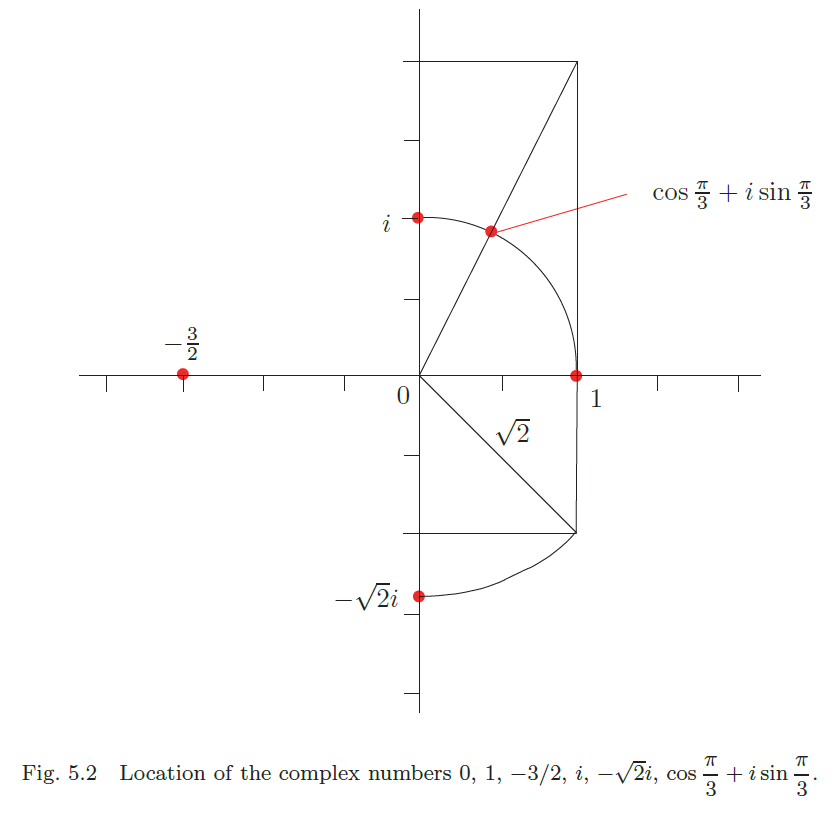
\includegraphics[width=0.7\textwidth]{./figs/fig-5-2}
\end{center}
\caption{복소수 $0$, $1$, $-3/2$, $i$, $-\sqrt{2}i$,
$\cos\dfrac\pi3 + i\sin\dfrac\pi3$의 위치}
\label{fig-5-2}
\end{figure}

\subsection*{연습문제 \ref{ex-1-5}}

$\theta\in\mathbb R$에 대하여
$(\cos\theta + i\sin\theta)^3 = \cos(3\theta) + i\sin(3\theta)$이다.
\begin{align*}
(\cos\theta + i\sin\theta)^3 
&= (\cos\theta + i\sin\theta)\left(
(\cos\theta)^2 - (\sin\theta)^2 + i2(\cos\theta)(\sin\theta) \right) \\
&= (\cos\theta)\left( (\cos\theta)^2 - (\sin\theta)^2 \right)
- (\sin\theta)2(\cos\theta)(\sin\theta)  \\
&\quad\quad + i(\ \cdots\ ).
\end{align*}
따라서 양변의 실수부가 같다는 것을 이용하면,
\begin{align*}
\cos(3\theta) &= \Re((\cos\theta + i\sin\theta)) \\
&=(\cos\theta)\left( (\cos\theta)^2 - (\sin\theta)^2 \right)
- 2(\cos\theta)(\sin\theta)^2 \\
&= (\cos\theta)\left( (\cos\theta)^2 - 1 + (\cos\theta)^2 \right)
- 2(\cos\theta)(1-\cos\theta)^2 \\
&= (\cos\theta)^3 - \cos\theta  + (\cos\theta)^3 - 2\cos\theta + 2(\cos\theta)^3 \\
&= 4(\cos\theta)^3 - 3\cos\theta
\end{align*}
다른 방법으로, 이항정리 공식
$(a+b)^n = \Sum_{k=0}^n \disp{n \choose k} a^kb^{n-k}$이
복소수 $a,b \in \mathbb C$와 자연수 $n\in \mathbb N$에 대하여
성립한다는 것을 이용하면,
\begin{align*}
\cos(3\theta) &= \Re((\cos\theta + i\sin\theta)) \\
&= \Re ( (\cos\theta)^3 + 3(\cos\theta)^2(i\sin\theta) 
+ 3(\cos\theta)(i\sin\theta)^2 + (i\sin\theta)^3) \\
&= (\cos\theta)^3 - 3(\cos\theta)(\sin\theta)^2 \\
&= 4(\cos\theta)^3 - 3\cos\theta.
\end{align*}

\subsection*{연습문제 \ref{ex-1-6}}

$1+i = \sqrt{2}\left(\dfrac1{\sqrt{2}} + i\dfrac1{\sqrt{2}}\right)
= \sqrt{2}\left( \cos\dfrac\pi4 + i\sin \dfrac\pi4 \right)$로 쓸 수 있다.
따라서,
\begin{align*}
(1+i)^{10}
&= (\sqrt{2})^{10} \left( \cos\dfrac\pi4 + i\sin \dfrac\pi4 \right)^{10}
= 2^5 \left( \cos\left(10\cdot \dfrac\pi4\right) 
+ i\sin \left(10\cdot \dfrac\pi4\right) \right) \\
&= 32 \left( \cos\left(2\pi+\dfrac\pi2\right) 
+ i\sin \left(2\pi+\dfrac\pi2\right) \right) \\
&=32 \left( \cos\left(\dfrac\pi2\right) + i\sin \left(\dfrac\pi2\right) \right) 
= 32(0+i\cdot 1) = 32i.
\end{align*}

\subsection*{연습문제 \ref{ex-1-7}}

$2+i$가 실수축의 양의 방향과 이루는 각도는 $\tan^{-1}(1/2)$이고
$3+i$가 실수축의 양의 방향과 이루는 각도는 $\tan^{-1}(1/3)$이다.
따라서, $(2+i)(3+i)$가 실수축의 양의 방향과 이루는 각도는 
$\tan^{-1}(1/2) + \tan^{-1}(1/3)$이다.
한편,
\[
(2+i)(3+i) = 6 - 1 + i(2+3) = 5 + 5i
\]
이므로 $(2+i)(3+i)$가  실수축의 양의 방향과 이루는 각도는
\[
\tan^{-1} (5/5) = \tan^{-1} 1 = \pi/4
\]
이다. 결론적으로, 
$\dfrac\pi4 = \tan^{-1}\dfrac12 + \tan^{-1}\dfrac13$이다.

\subsection*{연습문제 \ref{ex-1-8}}

정삼각형의 꼭지점  $A$, $B$, $C$의 위치가 
반시계방향의 순서로 복소수 $z_A$, $z_B$, $z_C$에 있다고 하자.
$\ell(AC) = \ell(AB)$이고 $\angle CAB=\pi/3$이므로,
\begin{equation}\label{eq-5-9}
z_C - z_A = \left( \cos\dfrac\pi3 + i\sin\dfrac\pi3 \right)(z_B - z_A).
\end{equation}
귀류법을 쓰기위해 $p,q,m,n\in\mathbb Z$가 
\[
z_C - z_A = p+iq, \quad
z_B - z_A = m+in
\]
을 만족한다고  하자.
그러면, 식 \eqref{eq-5-9}에서
$p+iq = \left(\dfrac12 + \dfrac{\sqrt{3}}2i\right)(m+in)$을 다시 쓰면,
\begin{align}
p &= \dfrac m2 - \dfrac{\sqrt{3}}2n, \label{eq-5-10} \\
q &= \dfrac{m\sqrt{3}}2 + \dfrac n2. \label{eq-5-11}
\end{align}
식 \eqref{eq-5-10}에 $-n$을 곱하고,
식 \eqref{eq-5-11}에 $m$을 곱하여 더하면,
\[
qm - pn = \dfrac{\sqrt{3}}2 (m^2 + n^2)
\]
을 얻는다.
그런데 $m^2+n^2 \ne0$이므로 ($z_B \ne z_A$이므로),
\[
\sqrt{3} = \dfrac{2(qm-pn)}{m^2+n^2} \in \mathbb Q
\]
를 얻어 모순이 생긴다.



